\documentclass[journal,12pt,twocolumn]{IEEEtran}

\usepackage{setspace}
\usepackage{gensymb}
\singlespacing
\usepackage[cmex10]{amsmath}

\usepackage{amsthm}
\usepackage{amsmath,amssymb}
\usepackage{mathrsfs}
\usepackage{txfonts}
\usepackage{stfloats}
\usepackage{bm}
\usepackage{cite}
\usepackage{cases}
\usepackage{subfig}

\usepackage{longtable}
\usepackage{multirow}
\usepackage{float}
\usepackage{enumitem}
\usepackage{mathtools}
\usepackage{steinmetz}
\usepackage{tikz}
\usepackage{circuitikz}
\usepackage{verbatim}
%\usepackage{tfrupee}
\usepackage[breaklinks=true]{hyperref}
\usepackage{graphicx}
\usepackage{tkz-euclide}
\usepackage{stackengine}
\usetikzlibrary{calc,math}
\usepackage{listings}
    \usepackage{color}                                            %%
    \usepackage{array}                                            %%
    \usepackage{longtable}                                        %%
    \usepackage{calc}                                             %%
    \usepackage{multirow}                                         %%
    \usepackage{hhline}                                           %%
    \usepackage{ifthen}                                           %%
    \usepackage{lscape}     
\usepackage{multicol}
\usepackage{chngcntr}
\usepackage{bm}
\DeclareMathOperator*{\Res}{Res}

\renewcommand\thesection{\arabic{section}}
\renewcommand\thesubsection{\thesection.\arabic{subsection}}
\renewcommand\thesubsubsection{\thesubsection.\arabic{subsubsection}}

\renewcommand\thesectiondis{\arabic{section}}
\renewcommand\thesubsectiondis{\thesectiondis.\arabic{subsection}}
\renewcommand\thesubsubsectiondis{\thesubsectiondis.\arabic{subsubsection}}
\newtheorem{lemma}{Lemma}
\newtheorem{sublemma}{Lemma}[lemma]

\hyphenation{op-tical net-works semi-conduc-tor}
\def\inputGnumericTable{}                                 %%

\lstset{
%language=C,
frame=single, 
breaklines=true,
columns=fullflexible
}
\makeatletter
\setlength{\@fptop}{0pt}
\makeatother
\begin{document}
\newtheorem{theorem}{Theorem}[section]
\newcommand{\BEQA}{\begin{eqnarray}}
\newcommand{\EEQA}{\end{eqnarray}}
\newcommand{\define}{\stackrel{\triangle}{=}}
\bibliographystyle{IEEEtran}
\raggedbottom
\setlength{\parindent}{0pt}
\providecommand{\mbf}{\mathbf}
\providecommand{\pr}[1]{\ensuremath{\Pr\left(#1\right)}}
\providecommand{\qfunc}[1]{\ensuremath{Q\left(#1\right)}}
\providecommand{\sbrak}[1]{\ensuremath{{}\left[#1\right]}}
\providecommand{\lsbrak}[1]{\ensuremath{{}\left[#1\right.}}
\providecommand{\rsbrak}[1]{\ensuremath{{}\left.#1\right]}}
\providecommand{\brak}[1]{\ensuremath{\left(#1\right)}}
\providecommand{\lbrak}[1]{\ensuremath{\left(#1\right.}}
\providecommand{\rbrak}[1]{\ensuremath{\left.#1\right)}}
\providecommand{\cbrak}[1]{\ensuremath{\left\{#1\right\}}}
\providecommand{\lcbrak}[1]{\ensuremath{\left\{#1\right.}}
\providecommand{\rcbrak}[1]{\ensuremath{\left.#1\right\}}}
\DeclarePairedDelimiter\ceil{\lceil}{\rceil}
\DeclarePairedDelimiter\floor{\lfloor}{\rfloor}
\theoremstyle{remark}
\newtheorem{rem}{Remark}
\newcommand{\sgn}{\mathop{\mathrm{sgn}}}
\providecommand{\abs}[1]{\vert#1\vert}
\providecommand{\res}[1]{\Res\displaylimits_{#1}} 
% \providecommand{\norm}[1]{\lVert#1\rVert}
%\providecommand{\norm}[1]{\lVert#1\rVert}
\newcommand{\norm}[1]{\left\lVert#1\right\rVert}
\providecommand{\mtx}[1]{\mathbf{#1}}
\providecommand{\mean}[1]{E[ #1 ]}
\providecommand{\fourier}{\overset{\mathcal{F}}{ \rightleftharpoons}}
%\providecommand{\hilbert}{\overset{\mathcal{H}}{ \rightleftharpoons}}
\providecommand{\system}{\overset{\mathcal{H}}{ \longleftrightarrow}}
	%\newcommand{\solution}[2]{\textbf{Solution:}{#1}}
\newcommand{\solution}{\noindent \textbf{Solution: }}
\newcommand{\cosec}{\,\text{cosec}\,}
\newcommand*{\permcomb}[4][0mu]{{{}^{#3}\mkern#1#2_{#4}}}
\newcommand*{\perm}[1][-3mu]{\permcomb[#1]{P}}
\newcommand*{\comb}[1][-1mu]{\permcomb[#1]{C}}
\newcommand\xrowht[2][0]{\addstackgap[.5\dimexpr#2\relax]{\vphantom{#1}}}
\providecommand{\dec}[2]{\ensuremath{\overset{#1}{\underset{#2}{\gtrless}}}}
\newcommand{\myvec}[1]{\ensuremath{\begin{pmatrix}#1\end{pmatrix}}}
\newcommand{\mydet}[1]{\ensuremath{\begin{vmatrix}#1\end{vmatrix}}}
\numberwithin{equation}{subsection}
\makeatletter
\@addtoreset{figure}{problem}
\makeatother
\let\StandardTheFigure\thefigure
\let\vec\mathbf
\renewcommand{\thefigure}{\theproblem}
\def\putbox#1#2#3{\makebox[0in][l]{\makebox[#1][l]{}\raisebox{\baselineskip}[0in][0in]{\raisebox{#2}[0in][0in]{#3}}}}
     \def\rightbox#1{\makebox[0in][r]{#1}}
     \def\centbox#1{\makebox[0in]{#1}}
     \def\topbox#1{\raisebox{-\baselineskip}[0in][0in]{#1}}
     \def\midbox#1{\raisebox{-0.5\baselineskip}[0in][0in]{#1}}
\vspace{3cm}
\title{Assignment 3}
\author{Chirag Mehta - AI20BTECH11006}
\maketitle
\newpage
\bigskip
\renewcommand{\thefigure}{\theenumi}
\renewcommand{\thetable}{\theenumi}
Download all the python codes from
\begin{lstlisting}
https://github.com/cmaspi/EE3900/tree/main/Assignment-3/Code
\end{lstlisting}
latex-tikz codes from 
\begin{lstlisting}
https://github.com/cmaspi/EE3900/blob/main/Assignment-3/main.tex
\end{lstlisting}
\section{Problem}
(Construction Q 2.14) Draw a circle of radius 3 units.
Take two points $\vec{P}$ and $\vec{Q}$ on one of its extended 
diameter each at a distance of $7$ units from its centre.
Draw tangents to the circle from these two points $\vec{P}$ and $\vec{Q}$ 
\section{Solution}
\begin{theorem}
  The points of intersection of the line 
\begin{align}
L: \quad \vec{x} = \vec{q} + \mu \vec{m} \quad \mu \in \mathbb{R}
\label{eq:conic_tangent}
\end{align}
with a general conic are given by
\begin{align}
\vec{x}_i = \vec{q} + \mu_i \vec{m}
\end{align}
%
where
\begin{multline}
\mu_i = \frac{1}
{
\vec{m}^T\vec{V}\vec{m}
}
\lbrak{-\vec{m}^T\brak{\vec{V}\vec{q}+\vec{u}}}
\\
\pm
{\small
\rbrak{\sqrt{
\sbrak{
\vec{m}^T\brak{\vec{V}\vec{q}+\vec{u}}
}^2
-
\brak
{
\vec{q}^T\vec{V}\vec{q} + 2\vec{u}^T\vec{q} +f
}
\brak{\vec{m}^T\vec{V}\vec{m}}
}
}
}
\label{eq:tangent_roots}
\end{multline}
\end{theorem}
The general form of a conic is given by
\begin{align}
  \vec{x}^T\vec{Vx}+2\vec{u}^T\vec{x}+f=0 \label{eq:conic}
\end{align}
for a circle, $\vec{V}=\vec{I}$ and $\vec{u}=-\vec{O}$ where $\vec{O}$ is the center of the circle.\\
Let $\vec{q}$ be the locus of the point of tangency from point $\vec{P}$, the distance of $\vec{P}$ from $\vec{O}$ is $d$ 
\begin{align}
  \vec{q-O}^T\vec{q-P}&=0\\
  \vec{q+u}^T\vec{q-P}&=0\\
  \vec{q}^T\vec{q}+\vec{u}^T\vec{q}-\vec{u}^T\vec{P}-\vec{q}^T\vec{P}&=0
\end{align} 
Using~\eqref{eq:conic}
\begin{align}
  (\vec{u+p})^T\vec{q}=-f-\vec{u}^T\vec{P}
\end{align}
Let $\vec{n}=\vec{u+P}$ and $c=-f-\vec{u}^T\vec{P}$
This is equation of a line, let $\vec{q}=\vec{a}$ be a point that lies on this line
\begin{align}
  \therefore \vec{q}=\vec{a}+\lambda\myvec{-\vec{e_1}^T\vec{n}\\\vec{e_2}^T\vec{n}}
\end{align}
We need to find the intersection point of this with the given circle.\\
Using~\eqref{eq:tangent_roots}
\begin{align}
  \vec{q} = \vec{a} + \mu_i \vec{m}
\end{align}
\begin{multline}
  \mu_i = \frac{1}
  {
  d^2
  }
  \lbrak{-\vec{m}^T\brak{\vec{a}+\vec{u}}}
  \\
  \pm
  {\small
  \rbrak{\sqrt{
  \sbrak{
  \vec{m}^T\brak{\vec{a}+\vec{u}}
  }^2
  -
  \brak
  {
  \vec{a}^T\vec{a} + 2\vec{u}^T\vec{a} +f
  }
  d^2
  }
  }
  }
\label{eq:sol}
\end{multline}
Now, we can confirm the solution by checking for $\vec{u}=\vec{0},\, \vec{P}=d\vec{e}_1,\, f=-r^2$
\begin{align}
  \implies \vec{n}=d\vec{e}_1,\, \vec{m}=d\vec{e}_2
\end{align}
An arbitrary choice of $\vec{a}$ could be $\frac{r^2}{d}\vec{e}_1$,
\begin{align}
  \mu_i &= \pm\frac{1}
  {
  d^2
  }
  {\small
  \sqrt{
  \brak{r^2d^2-r^4}
  }
  }\\
  \vec{q}&=\frac{r^2}{d}\vec{e}_1 \pm r \small\sqrt{1-\frac{r^2}{d}} \label{eq:pointOfTangency}
\end{align}



% \begin{lemma}
%   The points of contact for the tangent drawn from a point 
%   \begin{align}
%     \vec{P} = d\vec{e}_1, \text{ where } \vec{e}_1 = \myvec{1\\0}
%   \end{align}
%   to the circle are given by 
%   \begin{align}
%     \vec{x} = \frac{r^2}{d}\vec{e}_1  \pm r\sqrt{1 - \frac{r^2}{d^2}} \vec{e}_2 \label{eq:pointOfTangency}
%   \end{align}  
% \end{lemma}
% \begin{proof}
% If $\vec{x}$ be a point of contact for the tangent from $\vec{P}$, 
% \begin{align}
%   \vec{(P-x)}^T\vec{x}&=0 \\
%   \implies \vec{P}^{\top} \vec{x} &=\norm{\vec{x}}^2 = r^2\\
%   \implies \vec{e}_1^{\top} \vec{x} &= \frac{r^2}{d}
% \end{align}
% The above equation can be expressed in parametric form as 
% \begin{align}
%   \vec{x} = \frac{r^2}{d}\vec{e}_1 + \lambda \vec{e}_2
% \end{align}
% Substituting the above in 
% \begin{align}
%   \norm{\vec{x}}^2 = r^2,
% \end{align}
% yields
% \begin{align}
%   \norm{\frac{r^2}{d}\vec{e}_1 + \lambda \vec{e}_2}^2&=r^2\\
%   \implies \lambda^2 &= r^2\sbrak{1 - \frac{r^2}{d^2}}\\
%   \text{or, }\lambda &= \pm r\sqrt{1 - \frac{r^2}{d^2}}
% \end{align}
% \end{proof}
Let $\vec{A}, \vec{B}$ be the corresponding points of tangency from $\vec{P}=7\vec{e_1}$ and 
$\vec{C}, \vec{D}$ be the corresponding points of tangency from $\vec{Q}=-7\vec{e_1}$.\\
Using \eqref{eq:pointOfTangency}, we obtain all the points of tangency.

A plot for tangents is given below
\begin{figure}[!ht]
    \centering
    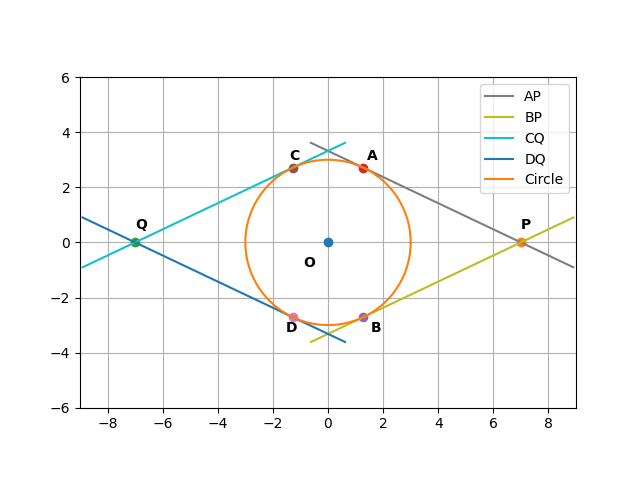
\includegraphics[width=\columnwidth]{plot/figure}
    \caption{Plot of the tangents}
    \label{plot}
\end{figure}
\end{document}